\chapter{ANÁLISE E DISCUSSÃO DE RESULTADOS}
\label{cap:resultados}
\renewcommand{\thetable}{\thechapter.\arabic{table}}
\renewcommand{\thefigure}{\thechapter.\arabic{figure}}
\setcounter{table}{0}\setcounter{figure}{0}
\section{Delimitação do experimento e critérios de comparação}
São avaliados dois cenários, com carteiras de uma a vinte ações,
sendo $n$ a quantidade de ações em cada carteira. No cenário de
ativos comuns, os dois modelos recebem o mesmo grupo de ações,
cuja composição permanece fixa durante o ano, e atualizam os
pesos mensalmente. No cenário de seleção própria, cada modelo
escolhe suas $n$ ações a cada rebalanceamento mensal. O primeiro
cenário compara a distribuição dos pesos entre as mesmas ações enquanto
o segundo avalia conjuntamente a escolha das ações e a
distribuição dos pesos. A Tabela~\ref{tab:configuracao_experimento}
resume a configuração geral do experimento.

\begin{table}[H]
\centering
\caption{Configuração geral do experimento.}
\label{tab:configuracao_experimento}
{\footnotesize
\renewcommand{\arraystretch}{0.85}
\begin{tabular}{p{0.40\linewidth}p{0.55\linewidth}}
\hline
Elemento & Configuração \\ \hline
Período avaliado & 250 pregões de 2025 \\
Capital inicial & R\$ 100.000 por simulação \\
Ações disponíveis & 20 ações \\
Quantidade de ações por carteira & De 1 a 20 \\
Modelos comparados & Black--Litterman e Markowitz \\
Comparação com as mesmas ações & 551 grupos de ações por modelo \\
Comparação com escolha própria & Cada modelo escolhe suas ações mensalmente \\
Atualização das carteiras & Mensal \\
Execução das operações & Fechamento do pregão seguinte ao sinal \\
Custo de negociação & 0,1\% sobre o volume negociado \\
\hline
\end{tabular}}
\par\smallskip{Fonte: Elaborado pelo autor.}
\end{table}

No cenário de ativos comuns, são avaliados todos os 20 grupos
possíveis com uma ação e todos os 20 grupos com dezenove ações,
além do único grupo com as vinte ações. Para cada quantidade
entre duas e dezoito ações, são sorteados 30 grupos distintos,
utilizando uma semente aleatória fixa para permitir a reprodução do
experimento. Ao todo, são 551 grupos de ações por modelo.

No cenário de seleção própria, são realizadas 20 simulações
por modelo, uma para cada quantidade de ações na carteira.
Somando os dois cenários, a comparação entre BL
e Markowitz compreende 1.142 simulações. Outras 1.142 simulações
avaliam duas configurações de referência: a expectativa de
equilíbrio sem opiniões adicionais e o uso direto das previsões
do XGBoost na otimização. Essas referências permitem examinar
a contribuição das etapas intermediárias para o resultado
financeiro.

\section{Desempenho quantitativo e escolha dos horizontes}
As previsões foram geradas pelo procedimento walk-forward, com
um modelo de regressão conjunto para as vinte ações em cada
horizonte e a identificação do ativo entre as variáveis de
entrada. Para cada ação, o horizonte foi definido com base na
acurácia direcional observada em 2024, considerando apenas
previsões cujos resultados já eram integralmente conhecidos
antes do início de 2025. Os horizontes assim definidos foram
mantidos durante a avaliação de 2025, sem ajustes baseados nos
resultados desse período. A Tabela~\ref{tab:previsoes_pool_2025} apresenta o diagnóstico do modelo conjunto nos horizontes utilizados na carteira. A coluna de validação descreve o pool em 2024, sem representar uma nova escolha de horizonte pelo maior acerto desse modelo. O número de pares avaliados por ativo em 2025 é 245, 240 ou 229 para horizontes de 5, 10 ou 21 pregões, respectivamente.

\begin{table}[H]
\centering
\caption{Desempenho das previsões utilizadas no experimento.}
\label{tab:previsoes_pool_2025}
{\footnotesize
\renewcommand{\arraystretch}{0.85}
\begin{tabular}{@{}cccccc@{}}
\hline
Ativo & $h$ & HR val. (\%) & HR 2025 (\%) &
\shortstack{Acurácia\\majoritária (\%)} & $R^2$ 2025 \\ \hline
ABEV3 & 5  & 42,68 & 49,39 & 49,80 & -0,017 \\
B3SA3 & 21 & 29,57 & 62,88 & 62,88 & -0,074 \\
BBAS3 & 10 & 41,57 & 50,00 & 50,42 & -0,034 \\
BBDC4 & 5  & 41,87 & 59,59 & 60,41 & -0,086 \\
CMIG4 & 21 & 71,30 & 65,94 & 65,94 & -0,029 \\
EQTL3 & 5  & 40,24 & 60,82 & 60,82 & -0,066 \\
GGBR4 & 21 & 63,91 & 61,57 & 61,57 & -0,013 \\
ITUB4 & 21 & 49,57 & 76,86 & 76,86 & -0,435 \\
LREN3 & 10 & 43,57 & 56,25 & 57,92 & -0,009 \\
MGLU3 & 21 & 56,52 & 59,83 & 52,40 & -0,027 \\
PETR3 & 10 & 57,68 & 43,75 & 52,92 & -0,025 \\
PETR4 & 21 & 54,78 & 48,47 & 51,53 & -0,057 \\
PRIO3 & 21 & 46,96 & 48,47 & 51,53 & -0,031 \\
RADL3 & 21 & 45,65 & 58,52 & 58,52 & 0,003 \\
RAIL3 & 21 & 37,83 & 44,98 & 55,02 & -0,041 \\
SANB11 & 21 & 39,78 & 64,19 & 64,19 & -0,139 \\
SBSP3 & 21 & 57,39 & 70,31 & 70,31 & -0,352 \\
SUZB3 & 10 & 54,36 & 37,08 & 62,92 & -0,082 \\
VALE3 & 10 & 43,82 & 70,83 & 71,25 & -0,151 \\
WEGE3 & 21 & 75,65 & 40,61 & 59,39 & -0,040 \\
\hline
\end{tabular}}
\par\smallskip
{\footnotesize {HR: acurácia direcional; $h$: horizonte em pregões;
Acurácia majoritária: acerto obtido ao prever sempre a classe
de retorno mais frequente em 2025.}}\\
Fonte: elaboração própria
\end{table}
\newpage
A média simples da acurácia entre ativos é 56,52\% em 2025. O contraste com a frequência da classe majoritária evidencia que acertar mais da metade das observações não assegura superioridade sobre uma referência trivial de sinal. A avaliação financeira exige, portanto, análise própria, sem transformar a acurácia em expectativa direta de retorno.

\subsection*{Horizontes utilizados e alcance do sinal preditivo}
\begin{table}[H]
\centering
\caption{Distribuição dos horizontes e diagnóstico agregado.}
\label{tab:diagnostico_pool}
{\footnotesize
\begin{tabular}{@{}p{0.47\linewidth}p{0.43\linewidth}@{}}
\hline
Indicador & Resultado \\ \hline
Horizonte de 5 pregões & 3 ativos (15\%) \\
Horizonte de 10 pregões & 5 ativos (25\%) \\
Horizonte de 21 pregões & 12 ativos (60\%) \\
Acurácia média em 2025 & 56,52\% \\
R$^{2}$ negativo em 2025 & 19 dos 20 ativos \\
HR acima da classe majoritária & 1 ativo; 8 empates; 11 abaixo \\
\hline
\end{tabular}}
\par\smallskip{Fonte: Elaborado pelo Autor.}
\end{table}
A predominância do horizonte de 21 pregões indica que o protocolo favorece sinais mais longos para a maior parte do universo, ainda assim, o desempenho das previsões variou entre as empresas. Os extremos do diagnóstico são ITUB4, com 76,86\% de acerto direcional, e SUZB3, com 37,08\%. Entretanto, ITUB4 apenas empata com a frequência da classe majoritária. MGLU3 é o único ativo que supera essa referência descritiva; oito ativos empatam e onze permanecem abaixo dela.

A acurácia direcional e o $R^2$ avaliam aspectos diferentes, um modelo pode acertar a direção do retorno e ainda errar sua
magnitude. O $R^2$ foi positivo apenas para RADL3, com valor
próximo de zero (0,0026). Para os demais ativos, o erro
quadrático das previsões foi maior que o obtido usando como
referência a média dos retornos observados em 2025. Essa média
é calculada após o período avaliado e serve apenas como
referência descritiva. Além disso, como os horizontes de
previsão se sobrepõem, previsões próximas compartilham dias
de retorno. Assim, uma acurácia superior a 50\% não demonstra,
por si só, significância estatística.

\subsection*{Erros de magnitude e coeficiente de determinação}
\begin{table}[H]
\centering
\caption{Métricas do XGBoost conjunto por horizonte em 2025.}
\label{tab:metricas_pool_horizontes}
{\footnotesize
\begin{tabular}{@{}rrrrrr@{}}
\hline
h & MAE & RMSE & HR (\%) & R$^2$ médio & Ativos com R$^2>0$ \\ \hline
5 & 3,10 & 4,09 & 53,92 & -0,0253 & 5 \\
10 & 4,54 & 5,81 & 56,21 & -0,0554 & 2 \\
21 & 6,72 & 8,42 & 58,41 & -0,1354 & 1 \\
\hline
\end{tabular}}
\par\smallskip{\footnotesize MAE e RMSE expressos em log-retorno multiplicado por 100.}
\\Fonte: Elaborado pelo Autor.
\end{table}
No horizonte de 21 pregões, o MAE foi de 6,72 e o RMSE de
8,42, expressos em log-retorno multiplicado por 100. O MAE
resume o tamanho médio dos erros absolutos, sem definir uma
faixa garantida em torno de cada previsão. O $R^2$ médio por
ativo permanece negativo nos três horizontes.

Ao reunir todas as observações das vinte ações e calcular
um único $R^2$ por horizonte, obtêm-se 0,0004, 0,0033 e
-0,0085 para 5, 10 e 21 pregões, respectivamente. Esse cálculo
difere da média dos coeficientes individuais apresentada na
tabela. Os valores agregados próximos de zero indicam erro
quadrático semelhante ao da referência baseada na média
geral dos retornos observados.

Em conjunto, os resultados indicam desempenho preditivo
limitado e variável entre os ativos, especialmente na
estimativa da magnitude dos retornos. Portanto, eventuais
resultados favoráveis das carteiras não constituem, por si
só, evidência da qualidade das previsões do XGBoost. Sua
interpretação deve considerar também o prior, a covariância,
as restrições de alocação e os custos de negociação.

\section{Qualidade da classificação de sentimento}

A classificação de sentimento foi avaliada em uma amostra
aleatória simples de 300 manchetes. Os rótulos definidos por
um avaliador humano, foram utilizados como referência para comparação
com o modelo. A concordância foi de 73,00\% (219 registros),
com macro-F1 de 72,19\% e kappa de Cohen de 0,595.

\begin{table}[H]
\centering
\caption{Desempenho da classificação de sentimento.}
\label{tab:sentimento_metricas}
{\footnotesize
\begin{tabular}{@{}lcccc@{}}
\hline
Classe & Suporte humano & Precisão (\%) &
Revocação (\%) & F1 (\%) \\ \hline
Positivo & 110 & 67,32 & 93,64 & 78,33 \\
Negativo & 73 & 73,91 & 93,15 & 82,42 \\
Neutro & 117 & 87,27 & 41,03 & 55,81 \\
\hline
\end{tabular}}
\par
Fonte: Elaborado pelo autor.
\end{table}

O modelo reconheceu mais de 93\% das manchetes positivas
e negativas da referência humana. A principal dificuldade
foi identificar as neutras: apenas 41,03\% receberam o mesmo
rótulo, enquanto as demais foram classificadas como positivas
ou negativas, conforme a Tabela~\ref{tab:sentimento_confusao}.

\begin{table}[H]
\centering
\caption{Matriz de confusão da classificação de sentimento.}
\label{tab:sentimento_confusao}
{\footnotesize
\begin{tabular}{@{}lccc@{}}
\hline
Humano / Modelo & Positivo & Negativo & Neutro \\ \hline
Positivo & 103 & 3 & 4 \\
Negativo & 2 & 68 & 3 \\
Neutro & 48 & 21 & 48 \\
\hline
\end{tabular}}
\par
Fonte: Elaborado pelo autor.
\end{table}

Esses resultados indicam maior atribuição de polaridade pelo
modelo em comparação com a referência humana, especialmente
positiva. A avaliação permanece limitada à amostra e ao
critério de um único avaliador com apoio de IA. Os indicadores
medem a concordância da classificação textual, sem demonstrar
a capacidade do sentimento de prever retornos ou melhorar
o desempenho das carteiras.
\section{Formação das views e cobertura informacional}
O experimento utiliza gate de três notícias: a presença de pelo menos três manchetes no dia elegível habilita a view híbrida. Abaixo desse limiar, o hard prior reduz sua confiança a um valor próximo de zero. Para avaliar a influência potencial das views, a auditoria deve incidir sobre as datas mensais de decisão, e não apenas sobre a cobertura diária do ano.

\begin{table}[H]
\centering
\caption{Cobertura nas datas de formação dos sinais mensais.}
{\footnotesize
\begin{tabular}{@{}rrr@{}}
\hline
Indicador & Quantidade & Percentual \\ \hline
Pares ativo-data avaliados & 240 & 100,00\% \\
Com alguma notícia no dia elegível & 40 & 16,67\% \\
Com ao menos três notícias (gate = 3) & 6 & 2,50\% \\
Abaixo do gate & 234 & 97,50\% \\
Datas mensais com alguma view elegível & 3 de 12 & 25,00\% \\
\hline
\end{tabular}}
\par
Fonte: Elaborado pelo Autor
\end{table}
O gate habilita 6 dos 240 pares ativo-data, presentes em 3 das doze datas mensais. Nas demais decisões, nenhuma ação atinge o mínimo de três manchetes. Esses números expressam cobertura informacional, não o tamanho exato da contribuição das views aos pesos. A regra é mais restritiva que a mera presença de uma notícia, embora quarenta pares contenham alguma manchete.

Nos ativos sem notícias elegíveis, a atualização permanece próxima do prior; nos demais, a mistura quantitativa e textual participa conforme a confiança estimada. A influência de uma opinião pode alcançar outros papéis pela estrutura de covariância. Por isso, o percentual de pares habilitados não deve ser interpretado diretamente como percentual da rentabilidade explicado pelas views.

A consulta apenas ao dia civil anterior ao sinal e a frequência mensal também limitam a informação utilizada: notícias em outros dias não geram rebalanceamento adicional. O gate de três foi adotado após a sensibilidade de 1 a 5 no próprio ano de 2025. Assim, o resultado descreve uma escolha retrospectiva, sem constituir validação independente do limiar nem evidência de irrelevância do sinal textual.

A Seção~\ref{sec:etapas_alocacao} apresenta a comparação
com o prior sem views e com as previsões do XGBoost
diretamente no otimizador. A avaliação preditiva a seguir
examina o efeito da polaridade textual nas expectativas
de retorno.

\section{Qualidade das views e da atualização Black--Litterman}

A análise compara as previsões de sete configurações:
XGBoost, Q completo, Q sem polaridade textual, BL com XGBoost,
BL sem polaridade, BL completo e prior sem views. O objetivo
é avaliar a contribuição do sentimento na formação de Q
e o efeito da atualização Black--Litterman sobre a qualidade
preditiva.

Nos controles sem polaridade, o sentimento é fixado em zero,
mantendo a contagem de notícias, os pesos quantitativos,
a matriz de incerteza e o gate de notícias. No controle
BL com XGBoost, Q recebe apenas a previsão quantitativa,
preservando as demais condições. Essas comparações permitem
examinar separadamente o efeito da polaridade textual e
da atualização pelo prior e pela covariância.

São avaliados 228 pares ativo-data de 2025 com retorno
realizado disponível no horizonte selecionado. Desses,
40 possuem notícias e 6 atingem o gate. O alvo utilizado
na avaliação é o retorno excedente diário equivalente:
\begin{equation}
\label{eq:alvo_diario_equivalente}
y_{i,t}^{(h)}
=
\frac{1}{h}
\ln\left(\frac{P_{i,t+h}}{P_{i,t}}\right)
-
r_{f,d},
\end{equation}
em que $P_{i,t}$ é o preço da ação $i$ na data $t$,
$h$ é o horizonte em pregões e $r_{f,d}$ é a taxa diária
livre de risco. A divisão por $h$ expressa o log-retorno
acumulado como uma média diária ao longo do horizonte.

Essa escala permite comparar XGBoost e Q com as expectativas
diárias do BL, mediante aproximação entre log-retornos
e retornos aritméticos. O HR mede o acerto do sinal do
retorno excedente à referência livre de risco.

A qualidade das previsões é avaliada pelo acerto direcional
(HR), pela acurácia balanceada (BA), pelos erros MAE e RMSE
e pelo coeficiente de determinação ($R^2$). A BA corresponde
à média das taxas de acerto das classes de sinal presentes.

\begin{table}[H]
\centering
\caption{Desempenho preditivo das configurações avaliadas.}
\label{tab:desempenho_camadas}
{\footnotesize
\renewcommand{\arraystretch}{0.85}
\begin{tabular}{@{}lcccccc@{}}
\hline
Previsão & N & HR (\%) & BA (\%) & MAE & RMSE & $R^2$ \\
\hline
XGBoost & 228 & 46,05 & 47,07 & 41,35 & 57,11 & -0,106 \\
Q sem polaridade & 228 & 46,05 & 47,22 & 41,30 & 56,88 & -0,097 \\
Q completo & 228 & 46,93 & 47,80 & 41,61 & 57,46 & -0,119 \\
BL com XGB & 228 & 53,07 & 50,11 & 39,60 & 54,23 & 0,003 \\
BL sem polaridade & 228 & 50,88 & 47,78 & 39,65 & 54,29 & 0,001 \\
BL completo & 228 & 55,70 & 52,37 & 39,20 & 53,82 & 0,018 \\
Prior & 228 & 54,39 & 50,00 & 39,47 & 54,18 & 0,005 \\
\hline
\end{tabular}}
\par\smallskip{\footnotesize
MAE e RMSE expressos em pontos-base por dia
(100 pontos-base = 1 ponto percentual).
}
\par
Fonte: Elaborado pelo autor.
\end{table}
O BL completo apresentou o menor RMSE, de 53,82 pontos-base,
e a maior acurácia direcional, de 55,70\%. Entretanto, sua
vantagem sobre o prior foi pequena, com redução de 1,34\% no
erro quadrático e aumento de 1,32 ponto percentual no HR.
\newpage
A Tabela~\ref{tab:efeitos_camadas} detalha as diferenças
entre as configurações.

\begin{table}[H]
\centering
\caption{Variação do desempenho entre configurações.}
\label{tab:efeitos_camadas}
{\footnotesize
\begin{tabular}{@{}lccc@{}}
\hline
Comparação & N & Redução MSE (\%) & Ganho HR (p.p.) \\
\hline
XGBoost $\rightarrow$ Q completo & 228 & -1,24 & 0,88 \\
Q sem polaridade $\rightarrow$ Q completo &
228 & -2,07 & 0,88 \\
BL sem polaridade $\rightarrow$ BL completo &
228 & 1,73 & 4,82 \\
XGBoost $\rightarrow$ BL com XGB & 228 & 9,81 & 7,02 \\
Q completo $\rightarrow$ BL completo & 228 & 12,28 & 8,77 \\
Prior $\rightarrow$ BL completo & 228 & 1,34 & 1,32 \\
\hline
\end{tabular}}
\par\smallskip{\footnotesize
As variações correspondem à passagem da primeira para
a segunda configuração (valores positivos indicam melhora)}\\
Fonte: Elaborado pelo autor
\end{table}

A inclusão da polaridade textual em Q aumentou o erro
quadrático em 2,07\%, embora tenha elevado o HR em
0,88 ponto percentual. Após a atualização BL, o efeito
foi favorável nos dois critérios: redução de 1,73\%
no erro e ganho de 4,82 pontos percentuais no HR.
O efeito do sentimento depende, portanto, de sua interação
com o prior e a covariância.

A atualização BL também melhorou a previsão quantitativa:
na comparação entre XGBoost e BL com XGB, o erro quadrático
caiu 9,81\% e o HR aumentou 7,02 pontos percentuais.

\begin{figure}[H]
\centering
\caption{Erro e acurácia balanceada das previsões
de cada camada.}
\label{fig:scores_camadas}
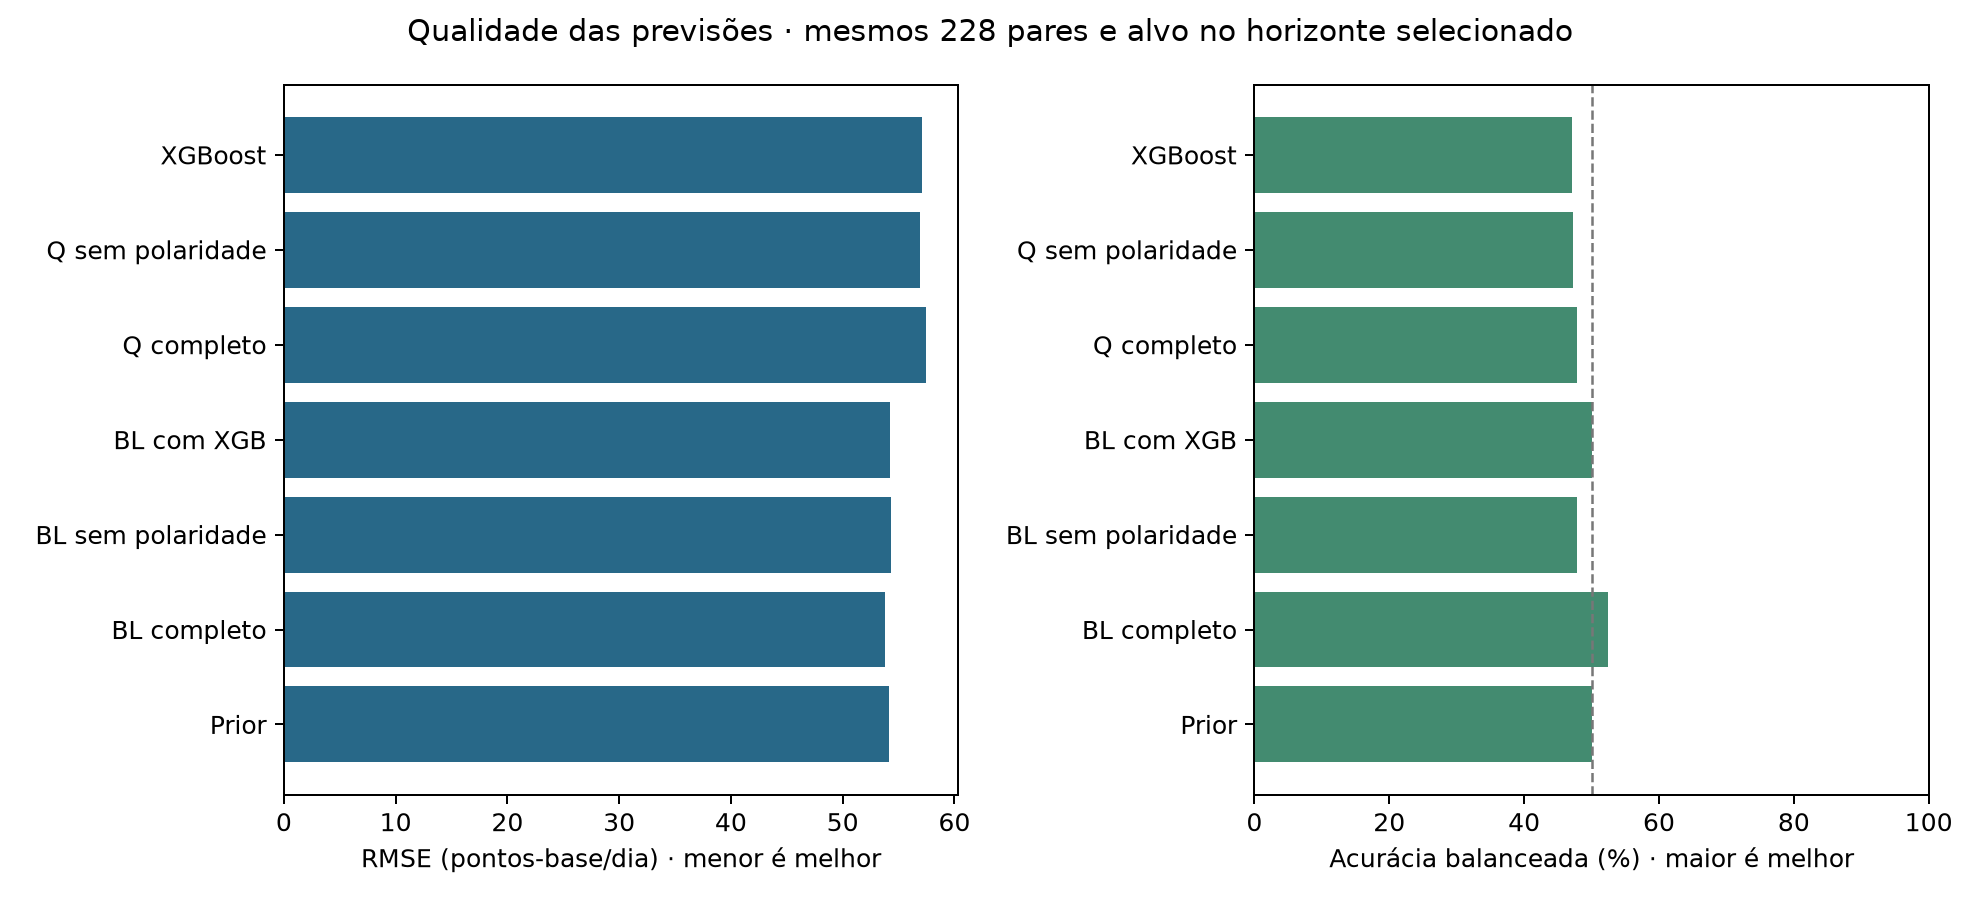
\includegraphics[width=\textwidth]
{05_Resultados/predicao_xgb/scores_camadas.png}
\par
Fonte: Elaborado pelo autor
\end{figure}

Entre os 40 pares com notícias, a inclusão da polaridade
textual apresentou o mesmo padrão: piora do erro em Q
e melhora após a atualização BL. As diferenças nesse
subconjunto são apresentadas na
Tabela~\ref{tab:efeitos_camadas_noticias}.

\begin{table}[H]
\centering
\caption{Variação do desempenho nas observações com notícias.}
\label{tab:efeitos_camadas_noticias}
{\footnotesize
\begin{tabular}{@{}lccc@{}}
\hline
Comparação & N & Redução MSE (\%) & Ganho HR (p.p.) \\
\hline
XGBoost $\rightarrow$ Q completo & 40 & -5,13 & 5,00 \\
Q sem polaridade $\rightarrow$ Q completo &
40 & -8,78 & 5,00 \\
BL sem polaridade $\rightarrow$ BL completo &
40 & 2,96 & 15,00 \\
XGBoost $\rightarrow$ BL com XGB & 40 & 6,44 & -10,00 \\
Q completo $\rightarrow$ BL completo & 40 & 13,17 & -12,50 \\
Prior $\rightarrow$ BL completo & 40 & 2,98 & 2,50 \\
\hline
\end{tabular}}
\par
Fonte: Elaborado pelo autor
\end{table}

Nesse subconjunto, a atualização de Q pelo BL reduziu
o erro quadrático em 13,17\%, mas diminuiu o HR em
12,50 pontos percentuais. Assim, a melhora na estimativa
da magnitude não foi acompanhada de maior acerto de direção.
A covariância também permite que uma view habilitada
altere as expectativas de outras ações no mesmo
rebalanceamento, estendendo seu efeito além dos ativos
com notícias.

\subsection{Sensibilidade à definição de previsão diária}

Como o BL trabalha na frequência diária, avalia-se também
o erro em relação ao retorno simples excedente do pregão
seguinte ao sinal, utilizando os 240 pares ativo-data
das decisões mensais. As previsões de XGBoost e Q são
convertidas da escala logarítmica diária equivalente para
a escala de retorno simples. O prior e o posterior são
utilizados como retornos simples excedentes.

Essa conversão permite comparar as configurações no mesmo
alvo diário, mas não transforma o XGBoost em um modelo
treinado para prever um único pregão. Por isso, os resultados
desta avaliação são apresentados separadamente daqueles
obtidos nos horizontes originalmente selecionados.

\begin{table}[H]
\centering
\caption{Desempenho preditivo no pregão seguinte ao sinal.}
\label{tab:desempenho_pregao_seguinte}
{\footnotesize
\renewcommand{\arraystretch}{0.85}
\begin{tabular}{@{}lcccccc@{}}
\hline
Previsão & N & HR (\%) & BA (\%) & MAE & RMSE & $R^2$ \\
\hline
XGBoost & 240 & 50,00 & 48,68 & 133,85 & 186,89 & -0,017 \\
Q sem polaridade & 240 & 49,17 & 47,65 & 133,85 & 186,92 & -0,017 \\
Q completo & 240 & 50,00 & 48,86 & 133,71 & 187,09 & -0,019 \\
BL com XGB & 240 & 46,67 & 50,42 & 133,69 & 185,80 & -0,005 \\
BL sem polaridade & 240 & 47,08 & 50,98 & 133,81 & 185,95 & -0,007 \\
BL completo & 240 & 49,17 & 53,40 & 133,34 & 185,48 & -0,002 \\
Prior & 240 & 44,58 & 50,00 & 134,00 & 186,14 & -0,009 \\
\hline
\end{tabular}}
\par\smallskip{\footnotesize
MAE e RMSE expressos em pontos-base por dia
(100 pontos-base = 1 ponto percentual).
}
\par
Fonte: Elaborado pelo autor.
\end{table}

O BL completo apresentou os menores erros, com MAE de
133,34 pontos-base e RMSE de 185,48 pontos-base, além da
maior acurácia balanceada, de 53,40\%. Sua acurácia direcional
foi de 49,17\%, abaixo dos 50,00\% obtidos pelo XGBoost
e por Q completo. O $R^2$ permaneceu negativo em todas
as configurações.

A inclusão da polaridade textual em Q reduziu ligeiramente
o MAE, mas aumentou o RMSE. No posterior BL, sua inclusão
reduziu ambos os erros e elevou o HR e a acurácia balanceada.
Assim, também no alvo diário, o efeito do sentimento variou
conforme a etapa em que foi avaliado.

\section{Avaliação das etapas de alocação}
\label{sec:etapas_alocacao}
São comparadas quatro configurações de alocação com vinte
ativos, mantendo-se o otimizador, as restrições, os custos
de transação e o calendário de rebalanceamento. O XGBoost
direto utiliza as previsões quantitativas sem atualização
pelo modelo Black--Litterman (BL), enquanto o prior sem
views utiliza apenas as expectativas de equilíbrio.

O índice de Sharpe mede o retorno excedente à referência
livre de risco por unidade de volatilidade. O drawdown
máximo (MDD) corresponde à maior queda percentual do
patrimônio em relação a um pico anterior e é apresentado
com sinal negativo.

\begin{table}[H]
\centering
\caption{Referências de alocação com vinte ativos.}
\label{tab:etapas_alocacao}
{\footnotesize
\renewcommand{\arraystretch}{1}
\begin{tabular}{@{}lrrrr@{}}
\hline
Configuração & Retorno (\%) & Sharpe & MDD (\%) & Custo (R\$) \\
\hline
BL híbrido       & 27,79 &  0,70 &  -8,46 & 507,76 \\
XGBoost direto   &  3,27 & -0,58 & -20,13 & 537,24 \\
Prior sem views  & 28,21 &  0,74 &  -8,46 & 135,07 \\
Markowitz        & 19,10 &  0,29 & -12,78 & 644,25 \\
\hline
\end{tabular}
}
\par\smallskip
{\footnotesize
O índice de Sharpe utiliza a Selic como referência, o retorno acumulado no período é de 14,87\%.
\par}
\smallskip
Fonte: elaboração própria
\end{table}

O XGBoost direto apresentou retorno inferior à Selic e
a maior queda máxima entre as configurações. O BL híbrido
superou tanto essa referência quanto Markowitz em retorno
e Sharpe, com menor queda máxima.

O prior sem views apresentou o maior retorno e Sharpe,
além do menor custo de negociação. Seu retorno superou
o do BL híbrido em 0,42 ponto percentual, indicando que,
na carteira de vinte ativos, a inclusão das views não
melhorou esses indicadores em relação ao uso exclusivo
das expectativas de equilíbrio.

\subsection*{Interpretação conjunta das etapas intermediárias}

A classificação de sentimento apresentou concordância de
73\% com a referência humana, com maior dificuldade na
identificação de manchetes neutras. Na avaliação preditiva,
a inclusão da polaridade textual aumentou o erro quadrático
de Q, mas reduziu o do posterior BL, indicando que seu efeito
depende da combinação com o prior e a covariância.

Na avaliação financeira com vinte ativos, o prior sem views
superou o BL híbrido em retorno e Sharpe. Assim, a melhora
preditiva observada após a atualização BL não foi acompanhada
de vantagem financeira sobre o prior nessa configuração.

\section{Comparação com ativos comuns}
A comparação pareada controla a composição elegível, os dois modelos recebem os mesmos ativos e operam nas mesmas datas. A diferença mediana é calculada primeiro dentro de cada par e depois agregada, ela pode diferir da subtração das duas medianas marginais. A Selic acumula 14,87\% nas 250 datas.

\begin{table}[H]
\centering
\caption{Retornos líquidos nos subconjuntos comuns.}
\label{tab:retornos_comuns}
{\footnotesize
\begin{tabular}{@{}rrrrrr@{}}
\hline
n & Conjuntos & BL med. (\%) & MV med. (\%) & $\Delta$ meadiano (p.p.) & $\mathrm{BL} > \mathrm{MV}$ (\%) \\ \hline
1 & 20 & 21,26 & 21,26 & 0,00 & 0,0 \\
2 & 30 & 21,81 & 21,81 & 0,00 & 0,0 \\
3 & 30 & 32,82 & 32,06 & 0,65 & 70,0 \\
4 & 30 & 29,14 & 21,03 & 9,00 & 90,0 \\
5 & 30 & 30,42 & 19,33 & 13,59 & 80,0 \\
6 & 30 & 31,22 & 14,56 & 11,92 & 80,0 \\
7 & 30 & 32,87 & 14,28 & 17,48 & 96,7 \\
8 & 30 & 32,97 & 15,44 & 18,78 & 93,3 \\
9 & 30 & 32,64 & 13,32 & 21,01 & 93,3 \\
10 & 30 & 33,08 & 11,01 & 19,92 & 90,0 \\
11 & 30 & 29,65 & 6,05 & 23,01 & 100,0 \\
12 & 30 & 34,47 & 12,61 & 22,20 & 96,7 \\
13 & 30 & 31,81 & 11,77 & 19,07 & 93,3 \\
14 & 30 & 30,77 & 18,85 & 10,84 & 90,0 \\
15 & 30 & 31,00 & 20,89 & 9,80 & 83,3 \\
16 & 30 & 30,35 & 16,00 & 16,29 & 96,7 \\
17 & 30 & 30,14 & 19,39 & 10,91 & 93,3 \\
18 & 30 & 28,40 & 19,35 & 10,53 & 100,0 \\
19 & 20 & 28,10 & 19,25 & 8,92 & 95,0 \\
20 & 1 & 27,79 & 19,10 & 8,69 & 100,0 \\
\hline
\end{tabular}}
\par\smallskip{\footnotesize
A última coluna mostra o percentual de grupos em que
BL obteve retorno superior
}
\par
Fonte: Elaborado pelo autor.
\end{table}

A vantagem do BL variou conforme a quantidade e a composição
das ações. Nas carteiras de cinco ativos, o modelo superou
Markowitz em 80,0\% dos grupos, com diferença mediana de
13,59 pontos percentuais. Com dez ativos, esses valores
foram de 90,0\% e 19,92 pontos percentuais, respectivamente.

\subsection*{Dispersão entre conjuntos e risco das carteiras}
\begin{figure}[H]
\centering
\caption{Retorno por cardinalidade com controle dos ativos elegíveis.}
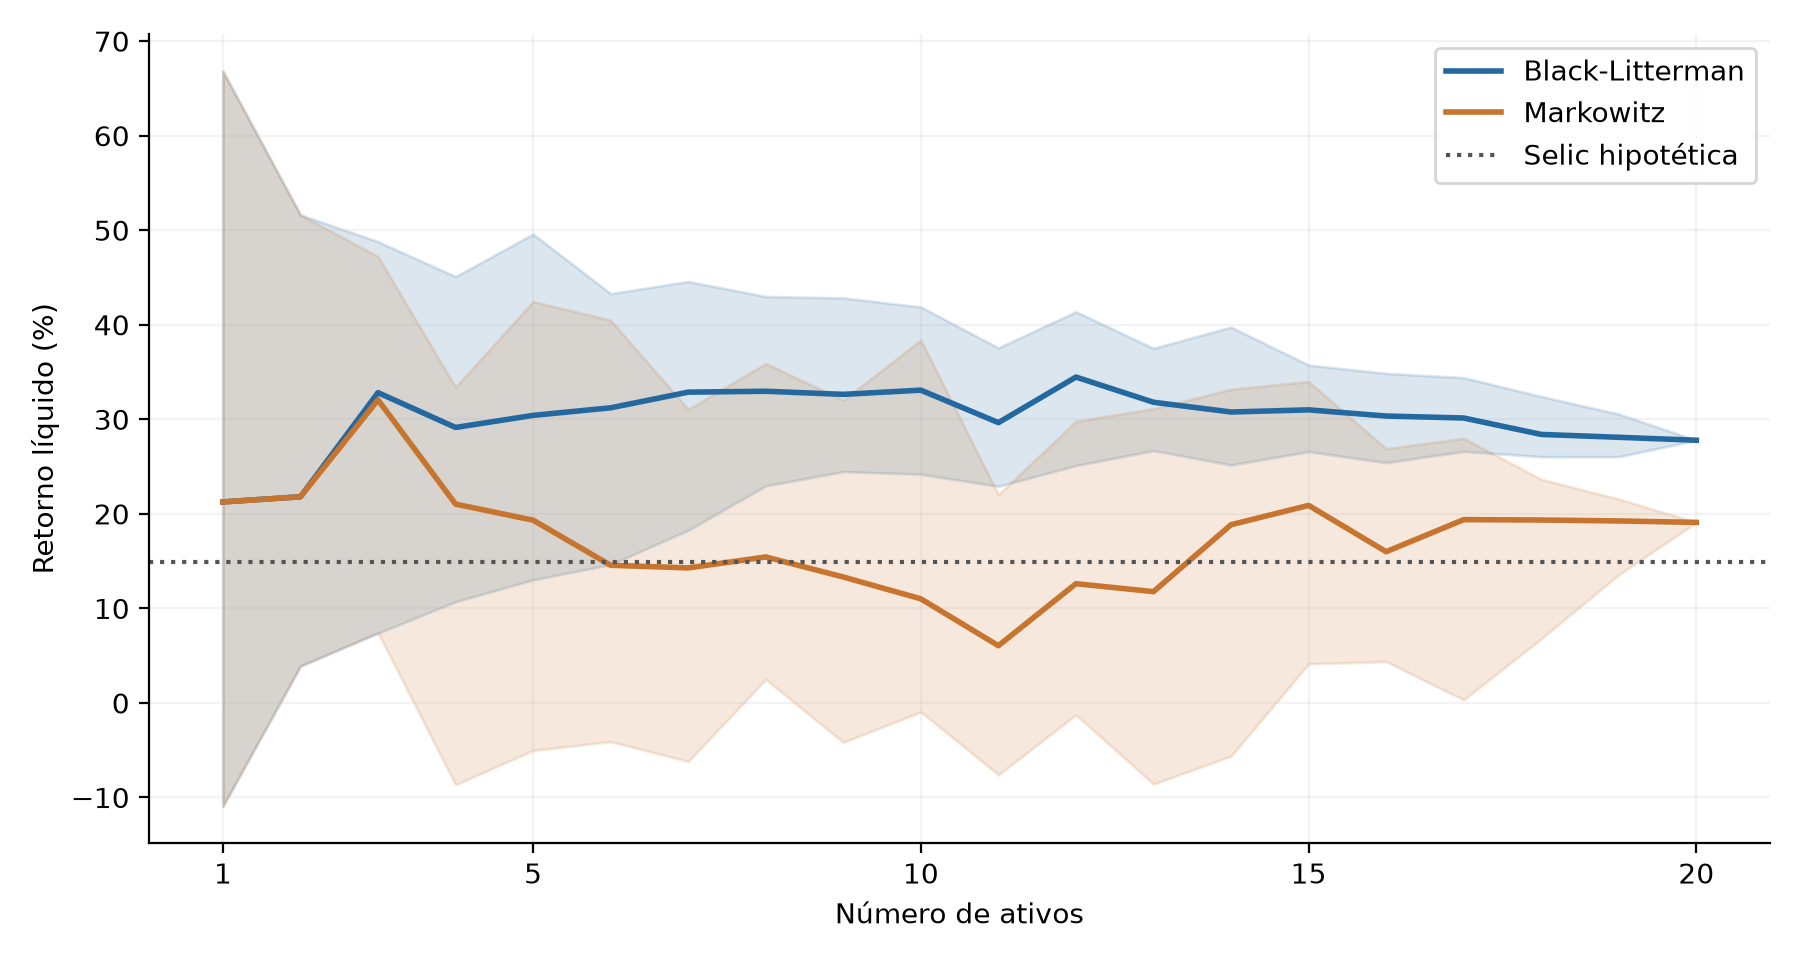
\includegraphics[width=\textwidth]{05_Resultados/figures/retorno liquido ativos.png}
Fonte: Elaborado pelo autor
\end{figure}
\begin{table}[H]
\centering
\caption{Risco e desempenho ajustado nos conjuntos comuns.}
\label{tab:risco_comuns}
{\footnotesize
\begin{tabular}{@{}rlrrr@{}}
\hline
n & Modelo & Sharpe med. & Volatilidade anual (\%) & MDD med. (\%) \\ \hline
1 & BL & 0,34 & 26,85 & -21,47 \\
1 & Markowitz & 0,34 & 26,85 & -21,47 \\
5 & BL & 0,78 & 18,65 & -9,34 \\
5 & Markowitz & 0,31 & 19,10 & -12,94 \\
10 & BL & 0,90 & 17,39 & -8,44 \\
10 & Markowitz & -0,05 & 19,40 & -18,19 \\
20 & BL & 0,70 & 17,49 & -8,46 \\
20 & Markowitz & 0,29 & 19,23 & -12,78 \\
\hline
\end{tabular}}
\par\smallskip{\footnotesize Cada coluna é uma mediana marginal e não representa necessariamente o mesmo subconjunto.}\\
Fonte: Elaborado pelo autor
\end{table}
No BL, o intervalo entre os percentis de retorno apresentados
foi de 13,01\% a 49,60\% nas carteiras de cinco ações e de
26,59\% a 35,74\% nas de quinze ações. A menor dispersão
com quinze ativos indica que, nos grupos avaliados, o
desempenho foi menos sensível à escolha das ações.

Com uma ação, os modelos apresentam resultados iguais,
pois investem todo o capital no mesmo ativo. Com duas,
o limite de 50\% por ação obriga a divisão igual dos pesos.
Com três, o teto de 34,17\% também mantém os pesos próximos
da divisão igual. Assim, nessas carteiras menores, os
limites de concentração reduzem a possibilidade de
diferenças entre as alocações dos modelos.

\section{Comparação com seleção própria dos ativos}
Na escolha livre, cada modelo ranqueia os ativos pelo retorno esperado excedente dividido pela volatilidade histórica. Markowitz utiliza a média móvel enquanto BL utiliza o posterior. A regra é explicitamente acrescentada à alocação e não corresponde à solução exaustiva do problema combinatório de selecionar a melhor carteira com n ações. Os retornos abaixo incluem seleção e distribuição de pesos.

\begin{table}[H]
\centering
\caption{Desempenho das estratégias com seleção própria.}
\label{tab:selecao_propria}
{\footnotesize
\begin{tabular}{@{}rrrrrrr@{}}
\hline
n & Ret. BL (\%) & Ret. MV (\%) & Sharpe BL & Sharpe MV & MDD BL (\%) & MDD MV (\%) \\ \hline
1 & -10,37 & 44,24 & -0,61 & 1,15 & -45,00 & -14,18 \\
2 & 77,64 & 32,41 & 1,53 & 0,83 & -24,22 & -11,16 \\
3 & 62,76 & 33,25 & 1,37 & 0,87 & -17,16 & -9,95 \\
4 & 62,27 & 23,33 & 1,59 & 0,46 & -12,62 & -11,94 \\
5 & 58,02 & 22,25 & 1,59 & 0,42 & -10,73 & -11,95 \\
6 & 49,43 & 20,07 & 1,36 & 0,33 & -10,68 & -12,68 \\
7 & 52,97 & 19,12 & 1,49 & 0,29 & -9,83 & -13,00 \\
8 & 46,08 & 18,78 & 1,31 & 0,27 & -8,20 & -13,00 \\
9 & 48,11 & 18,78 & 1,41 & 0,27 & -9,09 & -12,99 \\
10 & 43,72 & 18,84 & 1,27 & 0,27 & -9,16 & -12,97 \\
11 & 40,54 & 18,90 & 1,18 & 0,28 & -7,62 & -12,96 \\
12 & 40,46 & 18,88 & 1,19 & 0,28 & -7,57 & -12,95 \\
13 & 38,57 & 18,91 & 1,13 & 0,28 & -6,75 & -12,91 \\
14 & 33,46 & 18,96 & 0,92 & 0,28 & -6,73 & -12,89 \\
15 & 34,76 & 19,03 & 0,97 & 0,28 & -7,09 & -12,84 \\
16 & 34,40 & 19,09 & 0,97 & 0,28 & -7,28 & -12,82 \\
17 & 33,66 & 19,06 & 0,95 & 0,28 & -7,41 & -12,82 \\
18 & 32,48 & 19,05 & 0,90 & 0,28 & -8,04 & -12,82 \\
19 & 29,96 & 19,06 & 0,79 & 0,28 & -8,59 & -12,80 \\
20 & 27,79 & 19,10 & 0,70 & 0,29 & -8,46 & -12,78 \\
\hline
\end{tabular}}\\
Fonte: Elaborado pelo Autor
\end{table}
\newpage
BL supera Markowitz em retorno para 19 das 20 cardinalidades. Com uma ação, seu retorno é -10,37\%, contra 44,24\% de Markowitz, e seu drawdown é -45\%. Nesse caso, a distribuição de pesos é trivial, toda diferença decorre das ações escolhidas e das operações. A concentração exige atenção própria, mesmo quando carteiras maiores apresentam resultados favoráveis.

\subsection*{Trajetórias de capital e comparação com a renda fixa}
\begin{figure}[H]
\centering
\caption{Capital realizado em cardinalidades ilustrativas.}
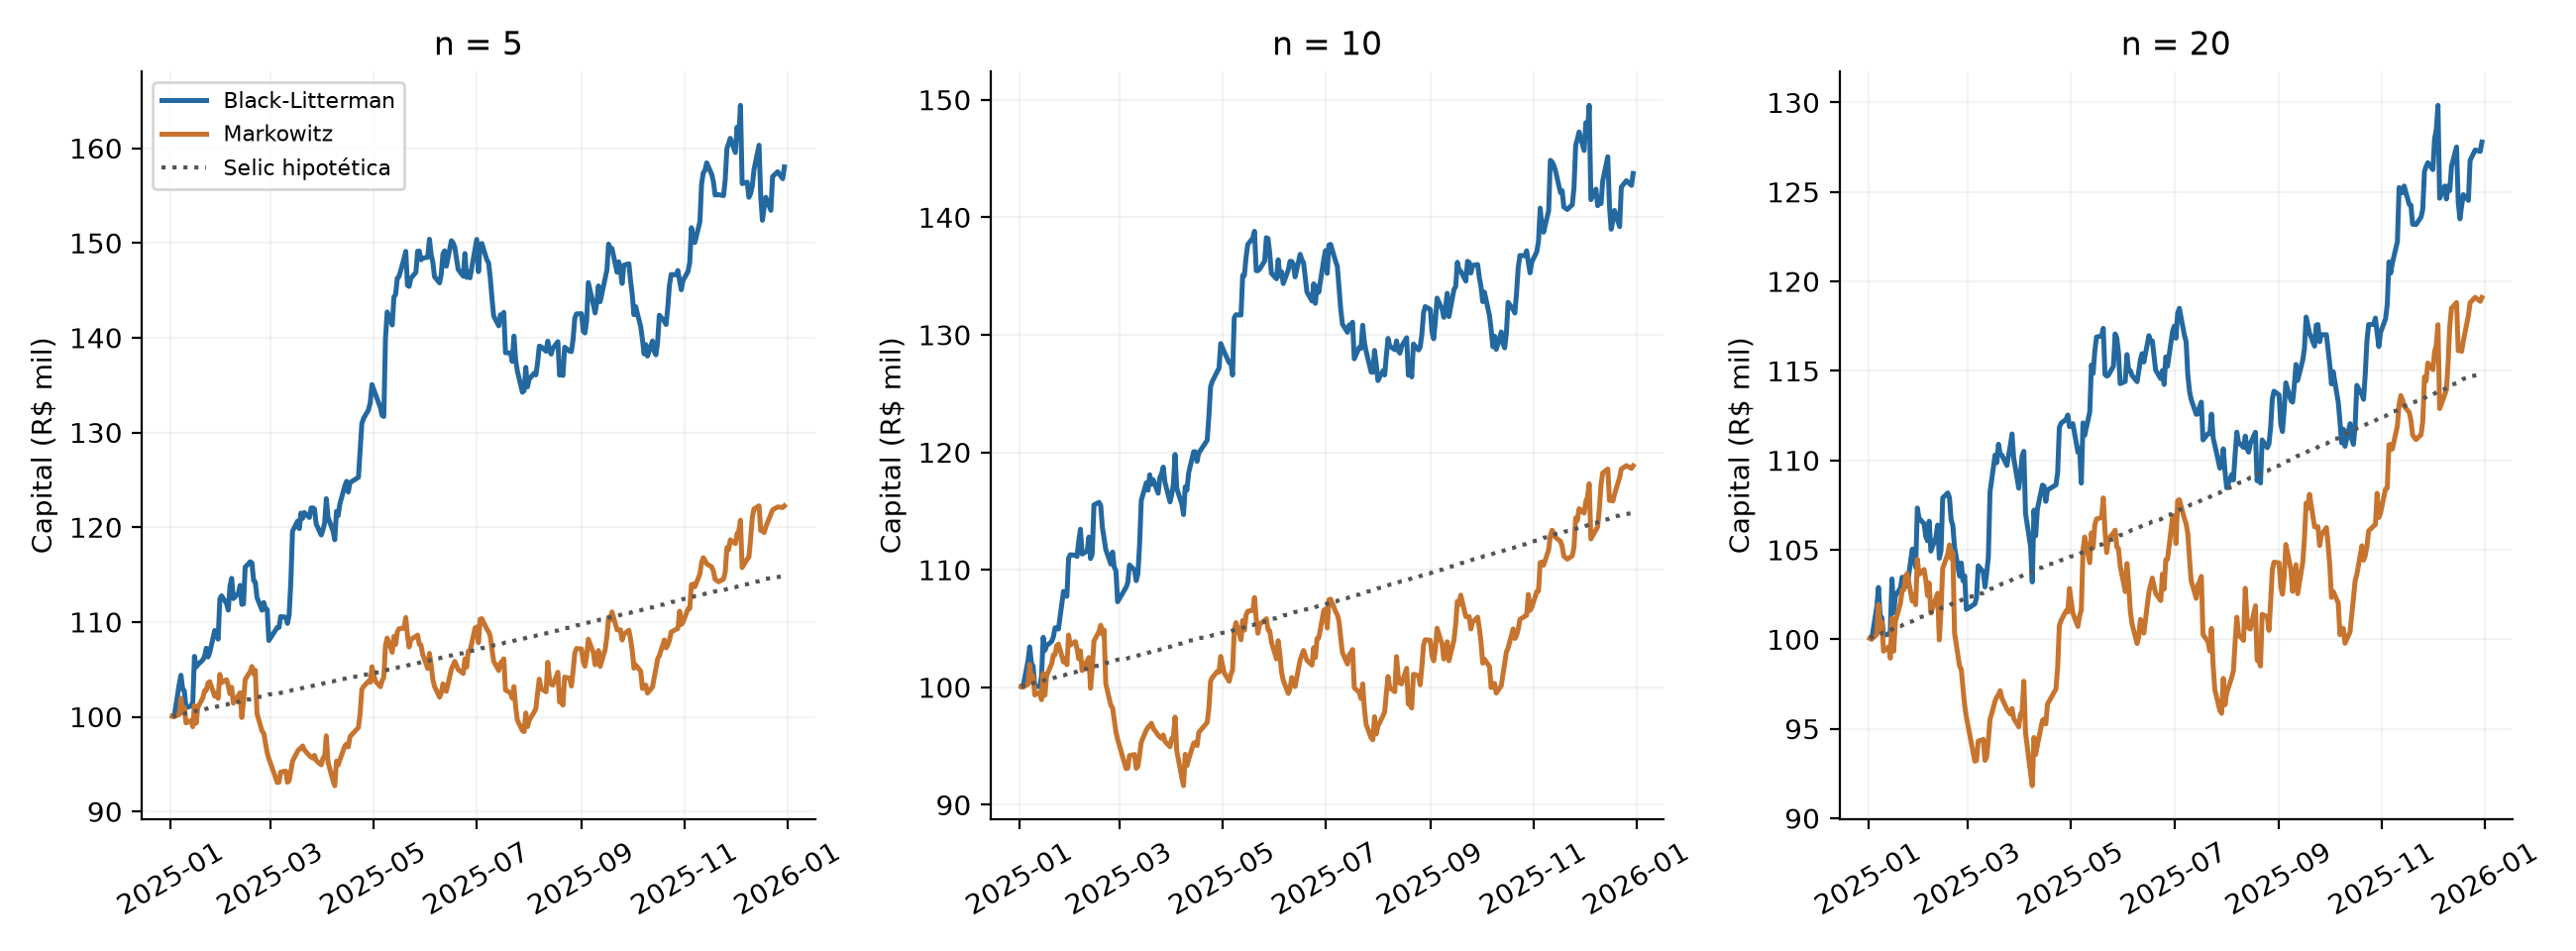
\includegraphics[width=\textwidth]{05_Resultados/figures/trajetoria de capital.png}
\par\smallskip{\footnotesize Capital inicial de R\$ 100 mil; custos de 10 bps}\\
Fonte: Elaborado pelo Autor
\end{figure}
\begin{table}[H]
\centering
\caption{Resultado com todo o universo de vinte ativos.}
\label{tab:universo_completo}
{\footnotesize
\begin{tabular}{@{}lrrr@{}}
\hline
Indicador & BL & Markowitz & Selic \\ \hline
Capital final (R\$) & 127.786,54 & 119.098,15 & 114.872,51 \\
Retorno líquido (\%) & 27,79 & 19,10 & 14,87 \\
Volatilidade anual (\%) & 17,49 & 19,23 & 0,00 \\
Sharpe sobre a Selic & 0,70 & 0,29 & Não definido \\
Drawdown máximo (\%) & -8,46 & -12,78 & 0,00 \\
\hline
\end{tabular}}
\par\smallskip{\footnotesize A Selic é uma série determinística, seu Sharpe não é definido por ter excesso e volatilidade nulos.}\\
Fonte: Elaborado pelo Autor
\end{table}
Em n = 20, os cenários coincidem, pois todos os ativos são elegíveis. A diferença de retorno BL menos Markowitz é 8,69 p.p., frente à Selic, é 12,91 p.p. As volatilidades são 17,49\% e 19,23\%, respectivamente. Essa comparação deve considerar também os drawdowns, pois a renda fixa não apresenta as oscilações das ações neste modelo simplificado.

O maior retorno de BL na escolha livre ocorre em n = 2, com 77,64\% e seu maior Sharpe ocorre em n = 5, com 1,59.

\section{Sensibilidade à cardinalidade e aos custos de transação}
Na seleção própria do BL, o retorno foi de -10,37\% com
uma ação, 77,64\% com duas e 27,79\% com vinte. Entre as
carteiras de uma e vinte ações, a volatilidade caiu de
32,48\% para 17,49\%. Entretanto, o retorno não aumentou
continuamente com a quantidade de ativos, pois cada tamanho
de carteira envolve diferentes ações selecionadas e
possibilidades de distribuição dos pesos.

\begin{table}[H]
\centering
\caption{Efeito dos custos nas estratégias com seleção própria.}
\label{tab:custos}
{\footnotesize
\begin{tabular}{@{}rlrrrr@{}}
\hline
n & Modelo & Sem custo (\%) & Líquido (\%) & Impacto (p.p.) & Custo pago (R\$) \\ \hline
1 & BL & -9,74 & -10,37 & 0,63 & 709,63 \\
1 & Markowitz & 45,25 & 44,24 & 1,01 & 735,18 \\
2 & BL & 79,27 & 77,64 & 1,63 & 1.318,63 \\
2 & Markowitz & 33,27 & 32,41 & 0,87 & 686,56 \\
5 & BL & 59,05 & 58,02 & 1,03 & 872,29 \\
5 & Markowitz & 23,01 & 22,25 & 0,76 & 639,14 \\
10 & BL & 44,59 & 43,72 & 0,86 & 756,24 \\
10 & Markowitz & 19,60 & 18,84 & 0,76 & 647,94 \\
20 & BL & 28,37 & 27,79 & 0,59 & 507,76 \\
20 & Markowitz & 19,85 & 19,10 & 0,75 & 644,25 \\
\hline
\end{tabular}}
\par\smallskip{\footnotesize
O resultado sem custos considera os mesmos pesos e operações
da simulação original, retirando apenas os custos de negociação.
}\\
Fonte: Elaborado pelo Autor
\end{table}
Os custos de negociação afetam o capital disponível para
os retornos seguintes. Por isso, o valor pago não corresponde
exatamente à redução do patrimônio final. Com vinte ações,
o BL pagou R\$ 507,76 em custos, reduzindo seu retorno em
0,59 ponto percentual. Markowitz pagou R\$ 644,25, com
redução de 0,75 ponto percentual. O giro da carteira
(\emph{turnover}) também foi menor no BL: 4,58, contra
6,30 de Markowitz.

Com duas ações, o BL apresentou turnover de 9,13 e custos
de R\$ 1.318,63, reduzindo o retorno em 1,63 ponto percentual.
Mesmo com pesos-alvo de 50\% para cada ação, a substituição
dos ativos selecionados e o ajuste dos pesos nos
rebalanceamentos geraram operações e custos.

\section{Limitações do experimento}

As simulações compartilham ações, datas e condições de
mercado, não constituindo observações independentes.
As medianas e as frequências de vitória descrevem os
grupos avaliados. Da mesma forma, o tamanho de carteira
com melhor desempenho em 2025 foi identificado
retrospectivamente.

A participação das views foi limitada pela cobertura
de notícias e apenas seis dos 240 pares ativo-data
atingiram o mínimo de três manchetes. Os controles
preditivos e financeiros permitem examinar etapas do
sistema, mas não separam integralmente a contribuição
de cada componente para a rentabilidade. A avaliação
do sentimento também utiliza uma referência definida
por um único avaliador humano com apoio de IA.

O universo fixo de ações está sujeito a viés de
sobrevivência e inclui diferentes classes de ações
da mesma empresa. A simulação considera execução no
fechamento seguinte ao sinal e custos proporcionais
ao volume negociado, sem incorporar spread, impacto
de mercado, tributação ou custos de encerramento
da carteira ao final do período.

Por fim, o prior utiliza pesos iguais entre os ativos,
em vez de ponderação por valor de mercado, e a conversão
das views para a escala diária é aproximada. A referência
livre de risco corresponde a uma taxa constante de
15\% ao ano, sem reproduzir a trajetória histórica
da Selic.